%%% use twocolumn and 10pt options with the asme2ej format
\documentclass[twocolumn,10pt]{wmrDoc}

\usepackage{epsfig} %% for loading postscript figures
\usepackage{hyperref}
\usepackage{parskip}
\hypersetup{colorlinks,linkcolor={black},citecolor={black},urlcolor={black}}  
\usepackage{graphicx} % Required for including images
\usepackage[font=small,labelfont=bf]{caption}
\hypersetup{colorlinks=true,urlcolor=black}
\usepackage{booktabs}       % professional-quality tables

%% The class has several options
%  onecolumn/twocolumn - format for one or two columns per page
%  10pt/11pt/12pt - use 10, 11, or 12 point font
%  oneside/twoside - format for oneside/twosided printing
%  final/draft - format for final/draft copy
%  cleanfoot - take out copyright info in footer leave page number
%  cleanhead - take out the conference banner on the title page
%  titlepage/notitlepage - put in titlepage or leave out titlepage
%  
%% The default is oneside, onecolumn, 10pt, final


\title{Detecting Evidence of Gender Discrimination in Fijian Court Documents}

%%% first author
\author{Chris Sexton and Greg Tozzi
    \affiliation{
    School of Information\\
	University of California, Berkeley\\
    email: cjsexton, greg.tozzi@ischool.berkeley.edu
    }	
}

\begin{document}

\maketitle    
%%%%%%%%%%%%%%%%%%%%%%%%%%%%%%%%%%%%%%%%%%%%%%%%%%%%%%%%%%%%%%%%%%%%%%
\begin{abstract}
{\it
Advances in natural language processing (NLP) and deep learning techniques provide practitioners with an expanded set of options for document classification. This paper leverages recent research in this area, applying convolutional neural networks and BERT variants against a challenging real world dataset to evaluate how well these approaches perform against traditional machine learning approaches.  We show that, for these data, state-of-the-art techniques can enjoy real advantages over more traditional techniques, but the effect is smaller than one might expect.
}
\end{abstract}

\section{Introduction}
This study considers the problem of identifying evidence of gender-based discrimination in Fijian court records for cases involving gender-based violence (GBV).  The problem of GBV in Fiji is serious and well documented, with 64\% of Fijian women reporting having experienced violence by an intimate partner.  The challenge of holding perpetrators accountable is sometimes confounded by an emphasis on the maintenance of the social order through blanket acceptance of traditional practices---referred to as \emph{vakaturaga}.  Traditional practices that make finding justice for survivors of GBV challenging include the patriarchal ordering of society---(\emph{matanitu})---and the practice of making atonement between men---(\emph{bulubulu}).  \emph{Bulubulu} involves making an offer of items of some value as a means of securing forgiveness and restoring of social harmony, but it is typically carried out by men and does not address the need and right of survivors to seek justice \cite{newland}.  Our work deals with finding evidence in texts generated by the Fijian judicial system that cultural norms have manifested as discriminatory practices in the courts.

The social benefits of detecting gender-based discrimination in court documents are clear.  Our natural language processing interest in studying this problem stems from the nature of the documents in question.  The court documents we examine in this study are relatively few in number, are of of arbitrary length, and are hand-coded by a small number of domain experts working for an international nongovernmental organization.  The small number of labeled documents (under 1,000), the wide range of document lengths (over 10,000 words), and the nuanced nature in the language used between discriminatory and non discriminatory documents, render the problem of classifying instances of gender based discrimination decidedly non-trivial.

We approached this problem wanting to know if state-of-the-art text classification methods offered substantially better performance over more established shallow and deep learning methods.  We explore the corpus in Section 2.  In Section 3 we conduct baseline studies using a shallow classifier.  In Section 4 we train convolutional neural networks with two different embedding schemes and apply them to the corpus.  In Section 5 we turn our attention to a variety of transformer models.  In Section 6 we consider the challenges specific to this corpus.  Section 7 deals with the problem of explainability.

\section{The Corpus}
Our data are provided by the International Center for Advocates against Discrimination (ICAAD), a non-governmental organization that conducts research and policy advocacy to combat structural discrimination. The data consist of 13,384 court documents from the Republic of Fiji. The documents cover a variety of matters. A subset of 809 documents involving cases of gender-based violence (GBV) are manually labeled with metadata indicating whether the document contains evidence of gender-based discrimination and, if it did, the form that the discrimination took. In general, appeals to outmoded cultural practices and ideas around gender roles that are used to justify a reduction in a perpetrator’s sentence are labeled as instances of discrimination.

Applying an 80/10/10 split, we divide the corpus into a training set of 647 documents and test and validations sets of 81 documents each.  Faced with a paucity of labeled documents, we weighed the benefits of removing the hold-out set entirely to maximize data available during model training.  Since many of our methods use validation loss during training as a trigger to adjust the learning rate, we determined that not presenting performance data on a hold out set would unacceptably limit the strength of our conclusions.

The lengths of documents in the corpus varies substantially as is shown in Table~\ref{tab:corpus}. Labels are applied to the entire document rather than the sentence level, so determining where offending text lies in the positively-labeled documents requires some degree of analysis.

\begin{table}
 \caption{Characteristics of the corpus}
  \centering
  \begin{tabular}{lrrrr}
    \toprule
    Subset   & Documents  & Avg length & 95\% & 99\%\\
    \midrule
    Complete & 13,384  & 2,218 & 5,989 & 11,259     \\
    Train    & 647  & 1,526 & 4,005 & 7,619      \\
    Test     & 162  & 1,414 & 3,320 & 7,203      \\
    \bottomrule
  \end{tabular}
  \label{tab:corpus}
\end{table}

The 809 documents related to GBV in the corpus contain labels for three sub-classes of gender discrimination.  The \emph{customary practices} label identifies instances in which methods of informal arbitration or restitution are improperly taken into account by the court.  The \emph{gender stereotypes} label indicates that the court has placed undue weight on perceived aspects of the victim's gender in forming its decision.  The third label is the catch-all \emph{other factors}.  The prevalence of each factor in the training and validation sets are shown in Table~\ref{tab:disc_type}.  Note that documents can be assigned more than one label.

\begin{table}
 \caption{Prevalence of discrimination factors}
  \centering
  \begin{tabular}{lrr}
    \toprule
    Factor   & Training  & Validation \\
    \midrule
    Customary practices & 0.25  & 0.25 \\
    Gender stereotypes  & 0.38  & 0.32 \\
    Other factors       & 0.28  & 0.31 \\
    \midrule
    Overall positive    & 0.58  & 0.59 \\
    \bottomrule
  \end{tabular}
  \label{tab:disc_type}
\end{table}

The corpus also contains a variety of document types.  These include decisions, rulings, sentencing documents, and judgements.  Each document type serves a different purpose, and some are specific to different parts of the judiciary.  Sentences, for instance, are specific to trial courts while judgements are issued by appellate courts. The document types exhibit different general structures and lengths.  The length of the documents in the training set disaggregated by document type are presented in Figure \ref{fig:boxplot}.

\begin{figure}[h]
    \centering
    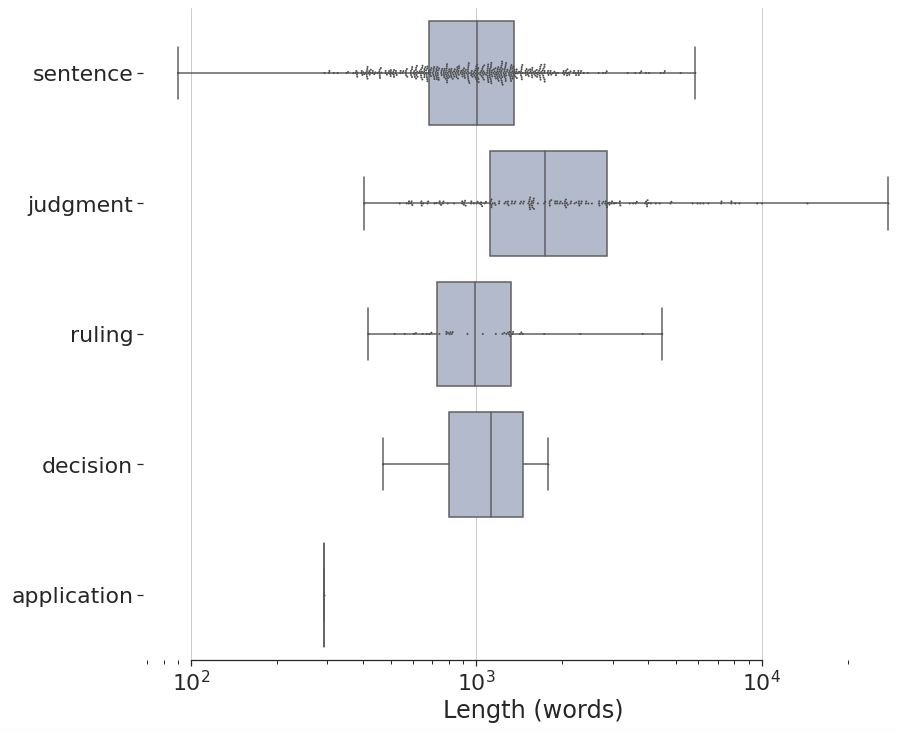
\includegraphics[width=.45\textwidth]{images/boxplot.png}
    \caption{Distribution of document lengths disaggregated by document type}
    \label{fig:boxplot}
\end{figure}

\section{Baseline Study - NBSVM}
To establish a performance baseline for binary classification, we examined classification performance using the naive Bayes support vector machine (NBSVM) classifier implemented in the ktrain library \cite{ktrain}.  The NBSVM model \cite{wang2012} seeks to balance the performance of multinomial naive Bayes and support vector machines for text classification.  The former are better suited for smaller sections of text while the latter perform better with longer sequences.  The model generates embeddings from naive Bayes log-count ratios and uses these as input to a support vector machine model.  The embeddings are fixed during training.

The NBSVM performed best with a maximum input length of 8,000 tokens.  We conducted training using ktrain's \verb|autotrain| function with a maximum learning rate of $10^{-4}$.  The \verb|autotrain| function automatically decreases the learning rate when it encounters a plateau in the validation loss.  Model performance was consistent for consecutive runs and is summarized in Table~\ref{tab:baseline}.

\begin{table}
 \caption{NBSVM average performance over four experiments}
  \centering
  \begin{tabular}{rrrr}
    \toprule
    Acc. & Precision & Recall & F1 \\
    \midrule
    0.70 & 0.90 & 0.66 & 0.77 \\
    \bottomrule
  \end{tabular}
  \label{tab:baseline}
\end{table}

Wang and Manning found that model performance increased when they trained with bigrams.  We did not find this to be the case for our corpus.  We ran related studies with a Fasttext-like model and a logistic regression model with trainable embeddings.  Both models performed slightly worse than the NBSVM model.

\section{Convolutional Neural Networks (CNNs)}
Kim demonstrated that relatively simple CNNs can achieve excellent results for sentence classification tasks \cite{kim}.  We explored the performance of CNNs on the task of classifying gender discrimination in our corpus using two models similar to Kim's.  The baseline architecture is shown in Figure \ref{fig:CNN}.  The unusual use of a two-element softmax classification head for a binary classification problem allows us to use the ktrain package and does not materially affect the model's results.  The model accepts 5,000 input word tokens per document, enough to ingest over 95\% of the documents in the corpus in their entirety.  Thirty-two filters each are learned for kernel sizes ranging from two to six.  The maximum activations of each filter---160 in all---are then concatenated and passed through a 64-neuron dense layer.

\begin{figure}[h]
    \centering
    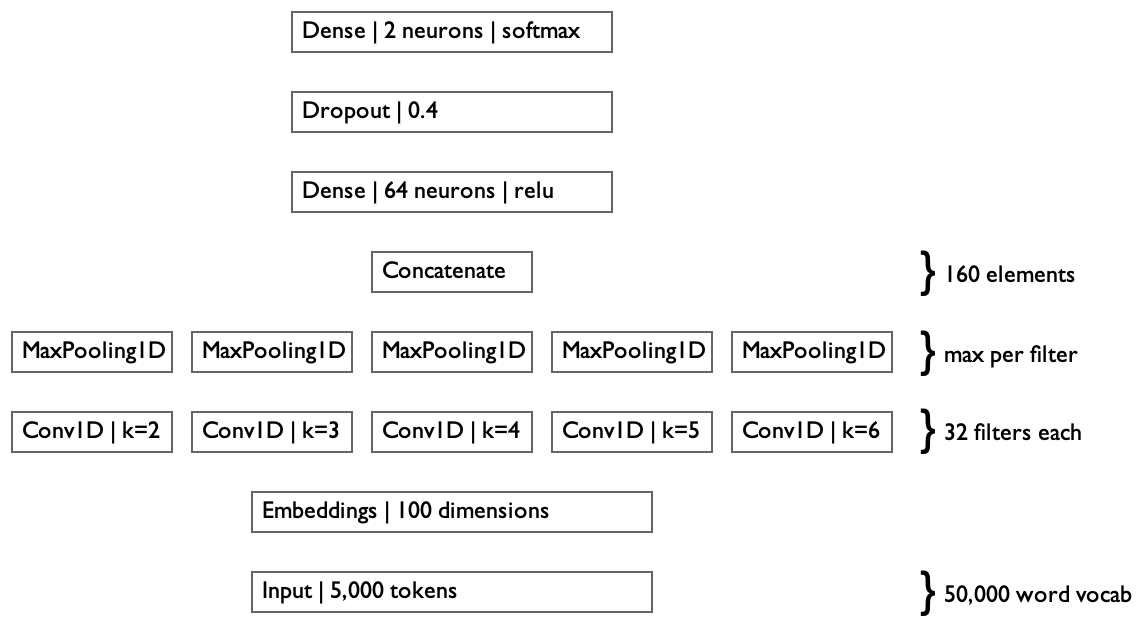
\includegraphics[width=0.48\textwidth]{images/CNN.png}
    \caption{Baseline CNN architecture showing a 100-dimensional embedding layer for the case of trainable embeddings}
    \label{fig:CNN}
\end{figure}

\subsection{CNN with trainable embeddings}
We implemented the model shown in Figure \ref{fig:CNN} which includes a randomly initialized 100-dimension word embedding layer at the bottom of the model.  Overfitting is a significant challenge, likely owing to the relatively small size of the data set which allowed the model easily to learn features unique to individual documents in the training set.  We managed overfitting by applying dropout regularization with a probability of 0.4 to the final dense hidden layer.  We also applied an implementation of the the triangular learning rate policy proposed by Smith \cite{smith2017} with a maximum learning rate of $10^{-3}$.  The training routine decreased the learning rate in response to plateaus experienced in the validation loss and applied early stopping when the model was no longer able to produce improvements in validation loss.

Training took roughly 64 second per iteration using an NVIDIA P6000 GPU.  Average model performance was not as good as NBSVM as detailed in Table~\ref{tab:cnn}.

The model encoded only a handful of meaningful semantic relationships in the learned embeddings.  For instance, \emph{bread} is closest to \emph{breadwinner} in terms of cosine similarity.  The terms \emph{breadwinner} and \emph{bread winner} are used interchangeably in several court documents, in the context of the traditional head of a Fijian household.  The majority of words in the vocabulary that we explored, however, did not have meaningful associations encoded in their embeddings except tangentially (\emph{daughter} was most closely associated with \emph{care}, for instance).

Noting that that models we built all had similar performance but tended to vary in individual predictions, we built a 10-learner bagged ensemble of CNNs \cite{goodfellow}.  The ensemble model's performance was substantially worse than that of the single model reported in Table~\ref{tab:cnn}. 

\subsection{CNN with domain-specific embeddings}
We used the full corpus of Fijian legal texts to build custom Word2Vec-style embeddings using the skip gram model provided by the \verb|gensim| package.  The resulting loya2Vec (loya being Fijian for lawyer) embeddings cover a vocabulary of nearly 33,000 words.  While the texts used to construct the embeddings include those in our training set, we purposefully excluded the texts contained in our validation and test sets from the embedding construction process.

As one might expect, semantic relationships are better captured in loya2Vec then they are in the embeddings learned in the previous section.  An sample of learned relationships is provided in Table~\ref{tab:loya2vec}.

\begin{table}
 \caption{Three closest neighbors using loya2Vec embeddings for a sample of words in the vocabulary}
  \centering
  \begin{tabular}{llll}
    \toprule
    Input       &  1 & 2 & 3\\
    \midrule
    breadwinner &  winner & bread & ilisavani\\
    victim      &  complainant & victim's & girl\\
    suva        &  labasa & lautoka & nausori\\
    sydney      &  brisbane & melbourne & perth\\
    \bottomrule
  \end{tabular}
  \label{tab:loya2vec}
\end{table}

Starting from the previous CNN architecture, we built the loya2Vec mapping into a new embedding layer.  As in the case of the CNN with trainable embeddings, the fixed-embedding model uses 32 filters each for kernel sizes two through six.  The model’s head consists of a 64-neuron dense layer to which a dropout probability of 0.4 is applied.  We were surprised to find that the loya2Vec-based CNN’s performance was not as good as was the model with a smaller trainable embedding layer as shown in Table~\ref{tab:cnn}.  We strongly suspect that this inversion of expected results is a consequence of the key characteristics of our data set---its small overall size and wide range of document lengths.

\begin{table}
 \caption{Average performance of CNN models across five experiments}
  \centering
  \begin{tabular}{lrrrr}
    \toprule
    Embeddings & Acc. & Precision & Recall & F1\\
    \midrule
    Trainable & 0.64 & 0.65 & 0.85 & 0.73 \\
    loya2Vec  & 0.63 & 0.67 & 0.77 & 0.71 \\
    \bottomrule
  \end{tabular}
  \label{tab:cnn}
\end{table}

\section{Transformers}
Bidirectional Encoder from Transformers \cite{devlin} represents recent development in deep learning techniques for NLP tasks. BERT has been trained on vast amounts of text and as such the BERT pre-trained language model can be used for classification tasks by simply applying a single additional linear layer to support the task. For the classification task the hidden state of the first token [CLS] is used as a representation of the entire sequence (document). 

BERT is designed to run against relatively small sequences of text, with a maximum length of 512 word pieces. Typically sentences or documents longer than this are truncated, potentially losing valuable signal information. Given the long form length of documents in the corpus, we implement a number of strategies designed to overcome the token limit.

For all experiments, we used the combined label for gender discrimination, and we used all document types. Sub-dividing the models or corpus with either of these factors returned lower accuracy and F1 scores than a combined approach.

The Huggingface library provides pre-trained BERT models as well as  variants of BERT such as DistilBert and Longformer which are used in these experiments. 

Firstly, we replicate two of the methods described by Sun et al \cite{sun}, specifically truncation methods and hierarchical methods. For the truncation approach input documents are truncated to provide smaller inputs, either by taking the first 512 or last 512 tokens. In this architecture the weights of the [CLS] token are jointly trained alongside the the parameter matrix for classification, maximizing the log probability for the correct label.

\begin{figure}[h]
    \centering
    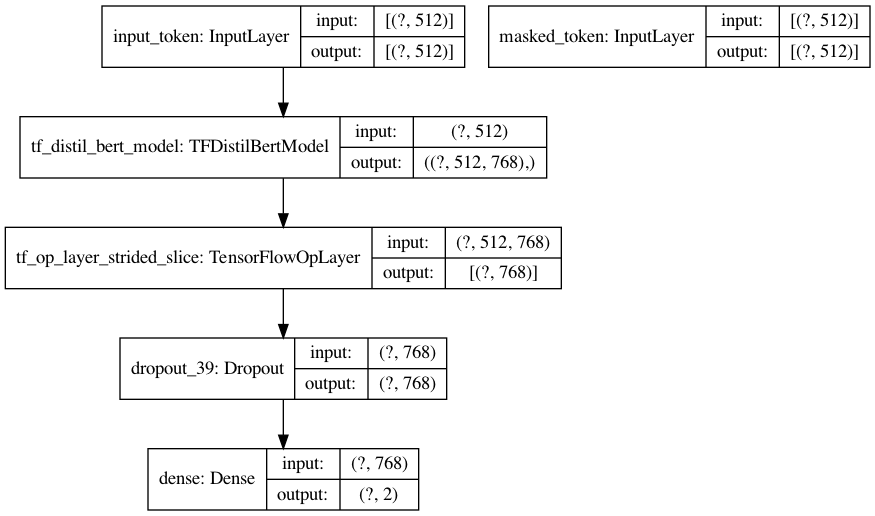
\includegraphics[width=0.48\textwidth]{images/DistilBert_TF.png}
    \caption{DistilBert Truncate Model}
    \label{fig:DistilBert}
\end{figure}

The hierarchical approach divides each document in $k = L/n$ segments where $n$ represents a specified maximum token length. At this point each document has been exploded to $\sum length(d)/n$ chunks.  Each resulting chunk may or may not contain signal to support its classification, therefore potentially confusing the model.  Two approaches to this concern are (a) to ignore it and assign the existing label to each chunk regardless, and (b) to freeze the embeddings for each chunk and aggregate the results across chunks for each document in a separate model. We tried both approaches but the latter was more effective, using an additional simple architecture of one $1000$ neuron $\tanh$ hidden layer and one dropout layer at $0.2$. We used a learning rate of $2e^{-5}$, $10$ epochs and batch size of $8$. Documents were split into 200 token chunks with 50 word overlaps prior to tokenization.  

Secondly we implement the method described by Pappagari et al \cite{Pappagari}, this takes a similar approach to the hierarchical method, however instead of pooling, the segment embedding outputs are stacked into a sequence which serves as input into a small (100 dimensional) LSTM layer. This is fed into two fully connected layers, a 30 dimensional RELU and then a softmax for the final classes. Embeddings are frozen prior to applying the LSTM.

The third and final approach is an implementation of Longformer, as described by Beltagy et al \cite{longformer}. Longformer has been trained on larger documents and can work with a word piece count of up to 4096. Longformer is not described in detail here, but in summary, it reduces the complexity of the self-attention component by sparsifying the full self-attention matrix according to an attention pattern, this is applied on a fixed sliding window. To improve task specific results, global attention is applied to specific input locations, in the case of classification this is the [CLS] token.

\subsection{Truncation, Hierarchical and Recurrent Methods }
We used DistilBERT and BERT pre-trained models to provide embeddings with a linear layer added for classification. Sanh et al \cite{sanh} provide a methodology, DistilBERT, that performs nearly as well as BERT but with lower computational cost. The DistilBERT architecture is identical to BERT's but differs by removing the token-type embeddings and the pooler, which are not needed for our classification task, and by reducing the number of layers from twelve to six. We conducted experiments with a batch size of eight---to conserve memory---over 3 epochs using the Adam optimizer and a learning rate of $2e^{-5}$.  This learning rate generally performed the best across BERT models. Training data was split 90/10 for training and validation.  Models are fine tuned on top of the pretrained  \verb|distilbert-uncased| model  with one additional linear layer on top of the [CLS] output embedding for classification.

Truncation methods on BERT were quite effective; using the last 512 tokens provided better results than using the head 512 tokens. This is not surprising as manual analysis of the text in which a judge evaluates mitigating factors---factors which frequently contain evidence of gender-based discrimination---generally appear toward the end of sentencing documents and judgements.  The documents in the corpus have already been pre-processed to remove non-useful header and tail information, so truncating the documents has a significant impact on signal processing.  Results returned from using the head and tail tokens are provided in Table~\ref{tab:headtail}. Averaged over five experiments, the tail approach gives an accuracy of 0.74 and an F1 of 0.74.

\begin{table}
 \caption{Results of applying truncation; three experiments each were conducted using head and tail tokens with batch size = 8, epochs = 3, and learning rate = $2^{-5}$}
  \centering
  \begin{tabular}{lrrrrr}
    \toprule
    Method & Acc. & Precision & Recall & F1\\
    \midrule
    Head & 0.64 & 0.69 & 0.64 & 0.62 \\
    Tail & 0.74 & 0.75 & 0.74 & 0.74  \\
    \bottomrule
  \end{tabular}
  \label{tab:headtail}
\end{table}

For the hierarchical models, mean and max pooling performed equivalently and worse than a simpler tail truncation approach.

Documents were split into 200 token chunks with 50 word overlaps prior to tokenization. 

\begin{table}
 \caption{Results of applying hierarchical approach. 5 runs of each set of experiments with finalized parameters of batch size=8 (1 for LSTM), epochs=5 (10 for aggregation, LSTM), learning rate of $2e^{-5}$ ($1e^{-5}$ for LSTM)}
  \centering
  \begin{tabular}{lrrrrr}
    \toprule
    Method & Acc. & Precision & Recall & F1\\
    \midrule
    Mean & 0.68 & 0.69 & 0.68 & 0.67 \\
    Max & 0.71 & 0.72 & 0.71 & 0.70  \\
    LSTM & 0.68 & 0.72 & 0.68 & 0.67  \\
    \bottomrule
  \end{tabular}
  \label{tab:hierarchical}
\end{table}

\subsection{Longformer Method}
The Longformer approach differs from the previous architectures in that it uses RoBERTa for tokenization and an alternative attention method. For pretraining, the weights from RoBERTa \cite{roberta} checkpoint are used, adding minimal changes required for attention (Beltagy et al. 2020). We utilize Longformer base consisting of 12 hidden layers and the Huggingface LongformerForSequenceClassification library which adds a Linear layer for classification.

Longformer was fine-tuned on two separate systems, one with a single NVIDIA K80 GPU and one with a single NVIDIA P100. Memory limitations prevented us from utilizing the full 4096 token segment length, even with 1024 tokens, the K80 was only able operate with a batch size of 1 (i.e. Stochastic gradient descent) whereas the P100 could operate a batch size up to 4. Multiple experiments were conducted with various learning rates, batch sizes and epochs. In all experiments a larger batch size was preferable over a larger segment length, and 3 epochs performed adequately. All Longformer methods were promising providing better results than the DistilBERT truncation and hierarchical methods. The best result is show in Table~\ref{tab:longformer_best} and more complete results are provided in Table~\ref{tab:longformer}.

\begin{table}
 \caption{Best Longformer result: batch size = 8, epochs = 3, and learning rate = $2^{-5}$}
  \centering
  \begin{tabular}{lrrrrr}
    \toprule
    Method & Acc. & Precision & Recall & F1\\
    \midrule
    Longformer & 0.71 & 0.72 & 0.84 & 0.78 \\
    \bottomrule
  \end{tabular}
  \label{tab:longformer_best}
\end{table}

\begin{table*}
 \caption{Longformer experiments with averaged results}
  \centering
  \begin{tabular}{rrrrrrrrr}
    \toprule
    Max Len & Epochs & Batch Size & LR & Experiments & Acc. & Precision & Recall & F1 \\
    \midrule
    512 & 5 & 8  & 2e-5 & 5 & 0.70 & 0.71 & 0.81 & 0.76 \\
    512 & 3 & 8  & 2e-5 & 1 & 0.69 & 0.71 & 0.81 & 0.76 \\
    512 & 5 & 8  & 4e-5 & 4 & 0.69 & 0.70 & 0.81 & 0.75 \\
    512 & 3 & 8  & 2e-5 & 2 & 0.71 & 0.72 & 0.84 & 0.78 \\
    512 & 3 & 12 & 2e-5 & 1 & 0.76 & 0.67 & 0.89 & 0.77 \\
    1024 & 3 & 6 & 2e-5 & 1 & 0.69 & 0.69 & 0.87 & 0.77 \\
    \bottomrule
  \end{tabular}
  \label{tab:longformer}
\end{table*}

For each experiment, the data was divided into 562 training samples, 65 validation samples and 162 test (holdout) samples. All experiments run with dropout 0.2 and attention dropout 0.2

Interestingly increasing batch size and token length has a slight improvement on F1 and recall but at the cost of precision. Considering the BERT variant models generally prefer to predict all positive results (higher recall) we need to be careful in evaluation. The practical implication of a false positive outweigh a false negative when classifying a court document as tainted by gender-based discrimination.

With more powerful compute it would be interesting to see if these results can be improved upon with the recommended batch size (16 or 32) and by utilizing more of the document text.

\section{Considering explainability}
While not a formal accusation of judicial misconduct, labeling a court document as containing evidence of bias certainly carries some weight.  Before applying a model to the task of potentially impugning the character of a sitting judge, we should provide a qualitative assessment of our predictions.  The LIME algorithm \cite{lime} provides a method for doing this via automated perturbation analysis.  In the case of text, LIME computes the sensitivity of a prediction to the input text by iteratively removing a single word from the input text and repeating the prediction.  

As an illustrative example, we consider the sentence \emph{As the accused is the sole breadwinner for his family, I reduce his sentence by two years.}  Taken by itself, and applying our understanding of ICAAD's concerns about Fijian jurisprudence, we expect that this sentence would be classified as containing evidence of gender based discrimination due to its appeal to the accused's patriarchal role in his family. Results are presented in Fig \ref{fig:LIME}.

\begin{figure}[h]
    \centering
    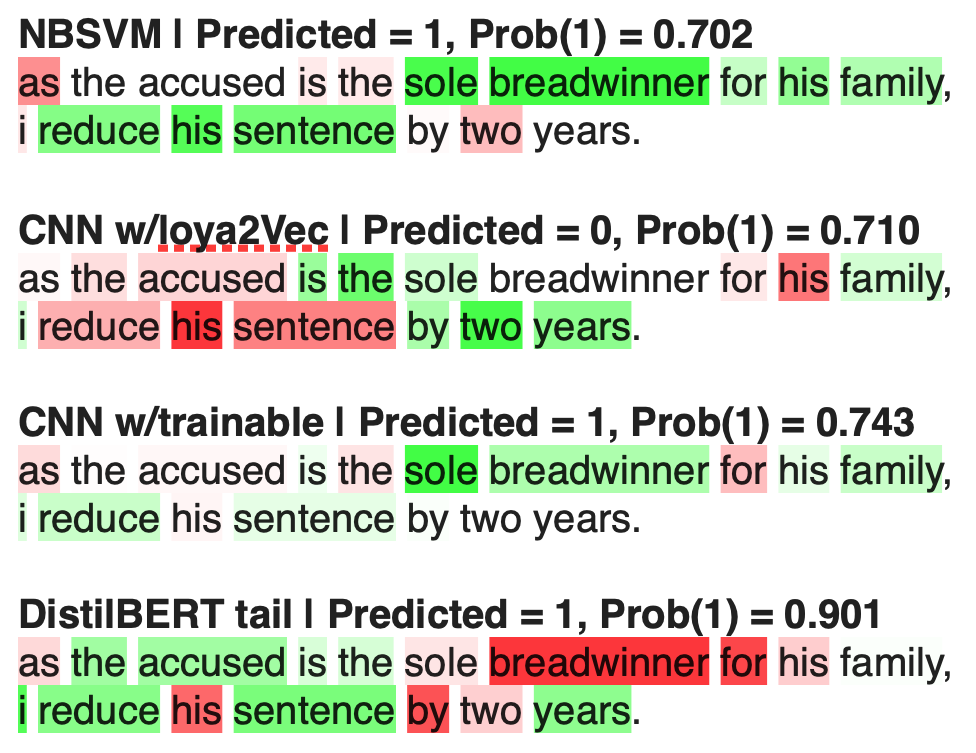
\includegraphics[width=0.4\textwidth]{images/LIME2.png}
    \caption{Application of the LIME algorithm to predictions generated by a variety of models}
    \label{fig:LIME}
\end{figure}

Green text in Figure \ref{fig:LIME} indicates words that support the classifer's prediction. The deeper the green, the stronger the impact of the highlighted word on the classification.  Red text similarly indicates words that did not support the prediction.  We see interesting differences in how the models treat the text.  The NBSVM produces the most reasonable output with the argument of the accused's position in his family and the resulting reduction in sentence identified.  The loya2Vec CNN gets the prediction wrong, but does identify the phrase \emph{reduce his sentence} as supporting a positive classification.  The CNN with trainable embeddings returns the correct class and identifies most of the loaded text.  The DistilBERT results are interesting and may be influenced by the model's word piece tokenization.

\section{Conclusions and next steps}

We attacked the problem of detecting gender discrimination in Fijian court documents with an array of methods, none of which returned the sort of results we had hoped to achieve, though the Longformer showed great promise.  Our consolidated results are presented in Table~\ref{tab:conclusion} for comparison.  No one measure of performance is sufficient to determine which classifier is the best.  If the classifier is going to be implemented in an automated system without much human review, accuracy and precision (to guard against false positives) should be carefully considered.  If the classifier is going to find itself in a system that triggers review by domain experts, accuracy and recall (to guard against false negatives) should be prioritized.

\begin{table*}
 \caption{Consolidated averaged results on the test set}
  \centering
  \begin{tabular}{lrrrrr}
    \toprule
    Method & Acc. & Precision & Recall & F1\\
    \midrule
    \em Transformers \\
    BERT w/tail truncation         & 0.74 & 0.75 & 0.74 & 0.74 \\
    BERT hierarchical max pooling  & 0.71 & 0.72 & 0.71 & 0.70 \\
    Longformer                     & 0.71 & 0.72 & 0.84 & 0.78 \\
    \midrule
    \em CNNs\\
    Trainable                      & 0.64 & 0.65 & 0.85 & 0.73 \\
    loya2Vec                       & 0.63 & 0.67 & 0.77 & 0.71 \\
    \midrule
    NBSVM                          & 0.70 & 0.90 & 0.66 & 0.77 \\
    \bottomrule
  \end{tabular}
  \label{tab:conclusion}
\end{table*}

Our results suggest the following conclusions and associated next steps:

1. The Longformer shows great promise, but our implementation was hampered by computational limitations.  Applying more compute to the problem should allow the Longformer model to ingest longer sections of text and return better results.

2. The challenges we experienced with managing overfitting suggests that our corpus is too small.  Additional document-level labeling by domain experts will likely improve model performance for subsequent efforts.

3. Heterogeneity in document length and structure makes this data set particularly challenging.  We tried several efforts to overcome this by steering our classifiers at the areas of the documents most likely to contain signal.  It may be insufficient to apply labels to long documents.  Subsequent efforts should include tagging---by domain experts---of sentences that contained evidence of gender-based discrimination.

4. There is still a place for simpler models.   Shallow models may outperform state-of-the-art methods when it comes to classifying documents that vary substantially in length and structure.  In particular, NBSVM produced results largely in line with more sohisticated methods.



%%%%%%%%%%%%%%%%%%%%%%%%%%%%%%%%%%%%%%%%%%%%%%%%%%%%%%%%%%%%%%%%%%%%%%



%%%%%%%%%%%%%%%%%%%%%%%%%%%%%%%%%%%%%%%%%%%%%%%%%%%%%%%%%%%%%%%%%%%%%%
\bibliographystyle{unsrt}  
%\bibliography{references}  %%% Remove comment to use the external .bib file (using bibtex).
%%% and comment out the ``thebibliography'' section.


%%% Comment out this section when you \bibliography{references} is enabled.
\begin{thebibliography}{1}

\bibitem{devlin}
Jacob Devlin, Ming-Wei Chang, Kenton Lee, and Kristina Toutanova.
\newblock Bert: Pre-training of deep bidirectional transformers for language understanding.
\newblock {\em arXiv preprint arXiv:1810.04805}, 2018.

\bibitem{roberta}
Yinhan Liu, Myle Ott, Naman Goyal, Jingfei Du, Mandar Joshi, Danqi Chen, Omer Levy, Mike Lewis, Luke Zettlemoyer, and Veselin Stoyanov.
\newblock Bert: RoBERTa: A Robustly Optimized BERT Pretraining Approach.
\newblock {\em arXiv preprint arXiv:1907.11692}, 2019.

\bibitem{sanh}
Victor Sanh, Lysandre Debut, Julien Chaumond, and Thomas Wolf.
\newblock DistilBERT, a distilled version of BERT: smaller, faster, cheaper and lighter.
\newblock {\em arXiv preprint arXiv:1910.01108}, 2019.

\bibitem{longformer}
Iz Beltagy, Matthew E. Peters, and Arman Cohan.
\newblock Longformer: The Long-Document Transformer.
\newblock {\em arXiv preprint arXiv:2004.05150}, 2020.

\bibitem{Pappagari}
Raghavendra Pappagari, Piotr Żelasko, Jesús Villalba, Yishay Carmiel, and Najim Dehak.
\newblock Hierarchical Transformers for Long Document Classification.
\newblock {\em arXiv preprint arXiv:1910.1078}, 2019.

\bibitem{sun}
Chi Sun, Xipeng Qiu, Yige Xu, and Xuanjing Huang.
\newblock How to Fine-Tune BERT for Text Classification?
\newblock {\em arXiv preprint arXiv:1905.05583}, 2019.

\bibitem{hadash2018estimate}
Guy Hadash, Einat Kermany, Boaz Carmeli, Ofer Lavi, George Kour, and Alon
  Jacovi.
\newblock Estimate and replace: A novel approach to integrating deep neural
  networks with existing applications.
\newblock {\em arXiv preprint arXiv:1804.09028}, 2018.

\bibitem{1607.01759}
Armand Joulin, Edouard Grave, Piotr Bojanowski and Tomas Mikolov.
\newblock Bag of Tricks for Efficient Text Classification, 2016;
\newblock arXiv:1607.01759.

\bibitem{kour2014fast}
George Kour and Raid Saabne.
\newblock Fast classification of handwritten on-line Arabic characters.
\newblock In {\em Soft Computing and Pattern Recognition (SoCPaR), 2014 6th
  International Conference of}, pages 312--318. IEEE, 2014.

\bibitem{newland}
Lynda Newland.
\newblock Villages, Violence and Atonement in Fiji.
\newblock In A. Biersack, M. Jolly and M. Macintyre (Eds.), {\em Gender Violence and Human Rights}, Australian National University Press, 2017.

\bibitem{smith2017}
Leslie N. Smith.
\newblock Cyclical Learning Rates for Training Neural Networks.
\newblock {\em arXiv:1506.01186v6}, 2017.

\bibitem{wang2012}
Sida Wang and Christopher Manning.
\newblock Baselines and Bigrams: Simple, Good Sentiment and Topic Classification.
\newblock In {\em Proceedings of the 50th Annual Meeting of the Association for Computational Linguistics (Volume 2: Short Papers)}, pages 90--94. Association for Computational Linguistics, 2012.

\bibitem{lime}
Marco Ribeiro, Sameer Singh and Carlos Guestrin.
\newblock “Why Should I Trust You?” Explaining the Predictions of Any Classifier.
\newblock {\em arXiv:1602.04938v3}, 2016.

\bibitem{ktrain}
Arun Maiya.
\newblock ktrain: A Low-Code Library for Augmented Machine Learning.
\newblock{\em arXiv:arXiv:2004.10703}, 2020.

\bibitem{kim}
Yoon Kim.
\newblock Convolutional Neural Networks for Sentence Classification.
\newblock{\em arXiv:1408.5882}, 2014.

\bibitem{goodfellow}
Ian Goodfellow, Yoshua Bengio and Aaron Courville.
\newblock \emph{Deep Learning}.
\newblock pp 249-251. MIT Press, 2016.

\end{thebibliography}

\end{document}